\documentclass[prl, reprint, final, showkeys]{revtex4-1}

\usepackage{amsmath}
\usepackage{amsfonts}

\usepackage{graphicx}
\usepackage{subcaption}

\usepackage{epstopdf}

\begin{document}


\title{Recovering System Dynamics using Diffusion Maps: A Chemotaxis Case Study}

\author{Carmeline J. Dsilva}
\email{cdsilva@princeton.edu}
\affiliation{Department of Chemical and Biological Engineering, Princeton University, Princeton, NJ, 08544}

\author{Ronen Talmon}
\email{ronen.talmon@yale.edu}
\affiliation{Department of Mathematics, Yale University, New Haven, CT, 06520}

\author{Ronald R. Coifman}
\email{coifman@math.yale.edu}
\affiliation{Department of Mathematics, Yale University, New Haven, CT, 06520}

\author{Ioannis G. Kevrekidis}
\email{yannis@princeton.edu}
\affiliation{Department of Chemical and Biological Engineering, Princeton University, Princeton, NJ, 08544}
\affiliation{Program in Applied and Computational Mathematics, Princeton University, Princeton, NJ, 08544}

\date{\today}

\begin{abstract}

Using a stochastic model which arises in cellular chemotaxis, we illustrate how manifold learning techniques, such as diffusion maps, can be used to characterize the behavior of a dynamical system.
%
In our model, depending on the value of a single parameter, the system dynamics at the macroscale range from heat equation dynamics, where particles diffuse uniformly outwards, to wave equation dynamics, where particle propagate with a fixed speed. 
%
We demonstrate that diffusion maps with the appropriate observers and metric can recover the two macroscopic system variables (initial condition and time) from data collected at the microscale in a variable- and equation-free manner. 
%
Furthermore, the order in which these variables are recovered is indicative of the system dynamics over the timescales of interest.
%
%We demonstrate that an essential component of our analysis is working with the right observers (histograms/ensembles, rather than the single position of a particle) and with the right metric between those observers (earth mover's distance, rather than Euclidean distance).
%
%In heat equation mode, we find that time is more important than the initial conditions, as the particles quickly equilibrate.
%
%In wave equation mode, we find that the initial conditions are more important, as the initial distribution simply propagates in time.
%	
%Furthermore, these two components have a completely different ``nature". 
%
%One parameter (the initial condition) is governing the entire trajectory and the other parameter (time) is governing the ``step­--by­--step" evolution within each trajectory.

\end{abstract}

\keywords{diffusion maps, earth mover's distance, histograms}

\maketitle

%\section{Introduction} 
 
Often, systems which are stochastic and noisy on the microscale exhibit smooth, coherent dynamics on the macroscale which are governed by only a few parameters.
%
For example, fluid flow, which can be described via the position and velocity of the fluid particles, is modeled at the macroscale using the Navier-Stokes equations.
%
However, in general, this mapping from microscale to macroscale is not always obvious.
%
We would like to {\em automatically} uncover the macroscale behavior from data collected at the microscale without knowing or assuming any microscopic or macroscopic model a priori.
%
TODO: write where this has been done in other places, context, etc.

In this letter, we will present how this goal can be achieved through a data-driven method based on geometric analysis and manifold learning. Specifically, we aim to emphasize two particular aspects of manifold learning from a dynamical systems' point of view: (a) the significance of the observers, especially in presence of noise and random dynamics, and (b) finding an appropriate metric of comparison. We will show that both are essential for our technique to successfully uncover the underlying dynamics of a given system.

We will illustrate our methodology through a model problem arising in studies of cellular chemotaxis \cite{othmer2000diffusion}.
%
In this example, the macroscopic dynamics vary depending on the value of a single system parameter.
%
We will demonstrate how we can use diffusion maps \cite{coifman2005geometric}, a manifold learning technique, to {\em automatically} detect changes in a system's macroscopic dynamics from microscale data.
%
This case study exhibits several key points which allow us to demonstrate the strength of our approach.
%
First, this system has random microscopic behavior with smooth macroscopic dynamics governed by few parameters, which determine the regime/mode of the system. 
%
Second, it consists of an ensemble of individual particles. 
%
Third, it has an analytic macroscopic description, which serves as a ground truth and will be used to verify our results, which will be obtained in an unsupervised manner.
%
We will show that diffusion maps based on statistical observers and the appropriate metric between them uncovers a description of the microscopic data which is consistent with the macroscopic model.
%
Furthermore, diffusion maps will uncover changes in dynamical behavior as we vary system parameters. 

The remainder of this letter is organized as follows. We will begin by describing the chemotaxis problem.
%
We will present the stochastic microscopic model, and show how, for this example, the microscopic model gives rise to a compact macroscopic description governed by a single parameter.
%
We will then use diffusion maps to analyze the microscopic simulation results, and show that using the appropriate metric for our data is essential to uncovering a meaningful description of our data.
%
Furthermore, we will show that diffusion maps can inform us as to the relative importance of system variables in different parameter regimes.

%\section{Problem formulation}

%\subsection{Chemotaxis ``story''} 

Chemotaxis is the movement of cells (such as bacteria) which is regulated by extracellular sensed signals.
%
These signals allow cells to accomplish tasks such as finding food and navigating away from toxins.
%
Several models have been proposed to describe the dynamics of cellular movement and dispersal \cite{othmer1988models, codling2008random}.
%
We will examine one such model described by a velocity jump process \cite{othmer2000diffusion}.
%
In this model, each cell is initialized with a position and a velocity, and the dynamics of each cell are governed by a stochastic process.
%
At random times, a cell will ``turn around'' and switch its velocity (this turning is controlled by extracellular signals). 
%
%We will analyze the dynamics of collections of such cells/particles. 

%\subsection{Stochastic particles}

We have a collection of $N$ particles whose states are defined by their positions and velocities. 
%
Let $x_i(t)$ and $v_i(t)$ denote the position and velocity, respectively, of particle $i$ at time $t$.
%
The velocity of each particle is either $\pm s$, where $s$ is a (fixed) speed. 
%
We initialize the particles such that
\begin{equation}
\begin{aligned}
x_i(0) & = 0 \\
\mathbb{P} \{ v_i(0) = +s \} & = p
\end{aligned}
\end{equation}
where $p$ is some probability.
%
The velocity of each particle randomly switches between $\pm s$ following an (independent) Poisson process with rate $\lambda$.
%
%Note that each particle has its own ``clock" (Poisson process).

%Let $X_{p, \lambda, s}(t)$ denote the vector of positions of the particles at time $t$ with initial right probability $p$, switching rate $\lambda$, and speed $s$.

For this specific example, we can write down explicitly the macroscopic equation that governs the overall system behavior.
%
For a large collection of particles ($N \rightarrow \infty$), the system can be described by the probability density of the particles.
%
Let $\rho(x, t)$ denote the probability density of the particles, and let $\rho^-(x, t)$ and $\rho^+(x, t)$ denote the densities of the particles moving towards the positive and negative axis directions, respectively.
%
It can be shown that, as $N \rightarrow \infty$, the densities obey the following set of partial differential equations (PDEs) \cite{othmer2000diffusion}:
\begin{equation} \label{eqn:coupled_pdes}
\begin{aligned}
\frac{\partial \rho^+}{\partial t} + s \frac{\partial \rho^+}{\partial x} & = -\lambda \rho^+ +\lambda \rho^- \\
\frac{\partial \rho^-}{\partial t} - s \frac{\partial \rho^-}{\partial x} & = \lambda \rho^+ -\lambda \rho^- 
\end{aligned}
\end{equation}
%
Alternatively, \eqref{eqn:coupled_pdes} can be rewritten as one, second--order PDE:
\begin{equation} \label{eq:second_order_pde}
\frac{\partial^2 \rho}{\partial t^2} + 2 \lambda \frac{\partial \rho}{\partial t} = s^2 \frac{\partial ^2 \rho}{\partial x^2}
\end{equation}
%
We assume that $s^2/\lambda = D$ is constant, so that the dynamics of the probability density are governed by a {\em single} parameter $\lambda$.

%\subsection{Asymptotic mode analysis}  \label{subsec:mode_analysis}

We will consider two regimes of simulation.
%
When $\lambda \rightarrow 0$, the right-hand side of \eqref{eqn:coupled_pdes} tends to 0, and \eqref{eqn:coupled_pdes} becomes two uncoupled wave equations,
\begin{equation}
\begin{aligned}
\frac{\partial \rho^+}{\partial t} + s \frac{\partial \rho^+}{\partial x} & = 0 \\
\frac{\partial \rho^-}{\partial t} - s \frac{\partial \rho^-}{\partial x} & = 0.
\end{aligned}
\end{equation}
%alternatively, \eqref{eq:second_order_pde} becomes the second order wave equation,
%\begin{equation}
%\frac{\partial^2 \rho}{\partial t^2} = s^2 \frac{\partial ^2 \rho}{\partial x^2}.
%\end{equation}

%Dividing \eqref{eq:second_order_pde} by $\lambda > 0$ yields
%\[
%\frac{1}{\lambda} \frac{\partial^2 \rho}{\partial t^2} + 2 \frac{\partial \rho}{\partial t} = D \frac{\partial ^2 \rho}{\partial x^2}
%\]
When $\lambda \rightarrow \infty$, \eqref{eq:second_order_pde} approaches the heat equation,
\begin{equation}
2 \frac{\partial \rho}{\partial t} = D \frac{\partial ^2 \rho}{\partial x^2}.
\end{equation}
%
This analysis implies that the initial distribution of the moving direction of the particles (given by $p$ in our microscopic simulations) plays a very different role depending on the value of $\lambda$.
%
When $\lambda \rightarrow 0$, the dynamics are described by two wave equations, and the initial distribution persists throughout the trajectory.
%
When $\lambda \rightarrow \infty$, the dynamics are described by one heat equation, and the initial conditions are insignificant -- the velocity distribution quickly equilibrates and we see purely diffusive behavior.
%
For this particular system, we can deduce this behavior from the macroscopic PDEs which describe the system dynamics.
%
However, we would like to demonstrate that, in general, these PDEs are not necessary for us to uncover which system variables are important to describe the macroscopic dynamics.
 

%\section{Methods and Analysis}

%\subsection{Diffusion maps}

We use diffusion maps \cite{coifman2005geometric} to analyze the data from simulations of the described microscopic stochastic model.
%
Our goal is to show that diffusion maps can organize the data obtained from the microscopic simulations, and that this organization is consistent with the two system variables, $p$ and $t$, that emerge from the PDE analysis.
%
Diffusion maps, in general, is a nonlinear manifold learning technique that embeds (maps) the data into a lower dimensional space. Ideally, the dimension of the embedded samples is equal to the the intrinsic (true) dimension of the data, and the variables/coordinates of the embedded samples represent the governing variables of the system.
%
In our case, although the data is very high-dimensional (e.g., the positions of all $N$ particles), for a fixed value of $\lambda$, there are only two important variables ($p$ and $t$) that determine the current (macroscopic) mode of the system; thus, our microscopic data {\em should} be two-dimensional and described by $p$ and $t$.
%
Let $z(t) \in \mathbb{R}^n$ denote an $n$-dimensional observation of the system at time $t$. Assume we are given $m$ observations $z(1), \dots, z(m)$, which are assumed to lie on a $d$-dimensional, nonlinear manifold, with $d \ll n$. Our goal is to uncover a $d$-dimensional parameterization of the $m$ observations that respects the underlying manifold geometry.
%
We first construct the matrix $W \in \mathbb{R}^{m \times m}$, with
\begin{equation} \label{eq:W}
W_{ij} = \exp \left( -\frac{\|z(i) - z(j) \|^2}{\epsilon^2} \right), \ i,j=1,\ldots,m
\end{equation}
where $\| \cdot \|$ denotes the appropriate norm for the data (which we will discuss in the following section), and $\epsilon$ is a characteristic distance between the observations (we take $\epsilon$ to be the median of the pairwise distances between the data points).
%
We then construct the diagonal matrix $D \in \mathbb{R}^{m \times m}$, with $D_{ii} = \sum_j W_{ij}$, and the matrix $A$, defined as
\begin{equation}
A = D^{-1} W.
\end{equation}
%
We compute the eigenvalues $\mu_0, \mu_1, \dots, \mu_{m-1}$ and eigenvectors $\phi_0, \phi_1, \dots, \phi_{m-1}$ of $A$, and order them such that $|\mu_0| \ge |\mu_1| \ge \dots \ge |\mu_{m-1}|$. 
%
Note that the matrix $A$ is row-stochastic ($\sum_j A_{ij} = 1$), which implies $\mu_0 = 1$ and $\phi_0$ is a constant vector.
%
The next few eigenvectors give us the embedding coordinates for our data;
$\phi_{j}(i)$ gives us the $j^{th}$ embedding coordinate for $z(i)$ and
$\mu_j$ gives a measure of the ``importance'' of coordinate $\phi_j$.

We first need to address what are the appropriate observers or measurements for our system.
%
Because the particles are indistinguishable, vectors containing the particle positions are not appropriate to analyze, as we would then be assigning indices or labels to the particles and swapping two particles would change the data.
%
Instead, we use histograms of the particle positions as our observables, so that $z(i) \in \mathbb{R}^n$ will be the histogram of $x_1(i), x_2(i), \dots, x_N(i)$ into $n$ bins (for our simulations, we take $n=32$).
%
Clearly, histograms are invariant to the labeling or indexing of the particles.
%
For this particular example, using histograms is consistent with our macroscopic PDE description, which is written in terms of the probability density of the particles.
%
The histograms serve as an empirical estimate of the probability density at each time point.

%\subsection{Earth mover's distance}

\begin{figure}[t]
\begin{subfigure}{0.2\textwidth}
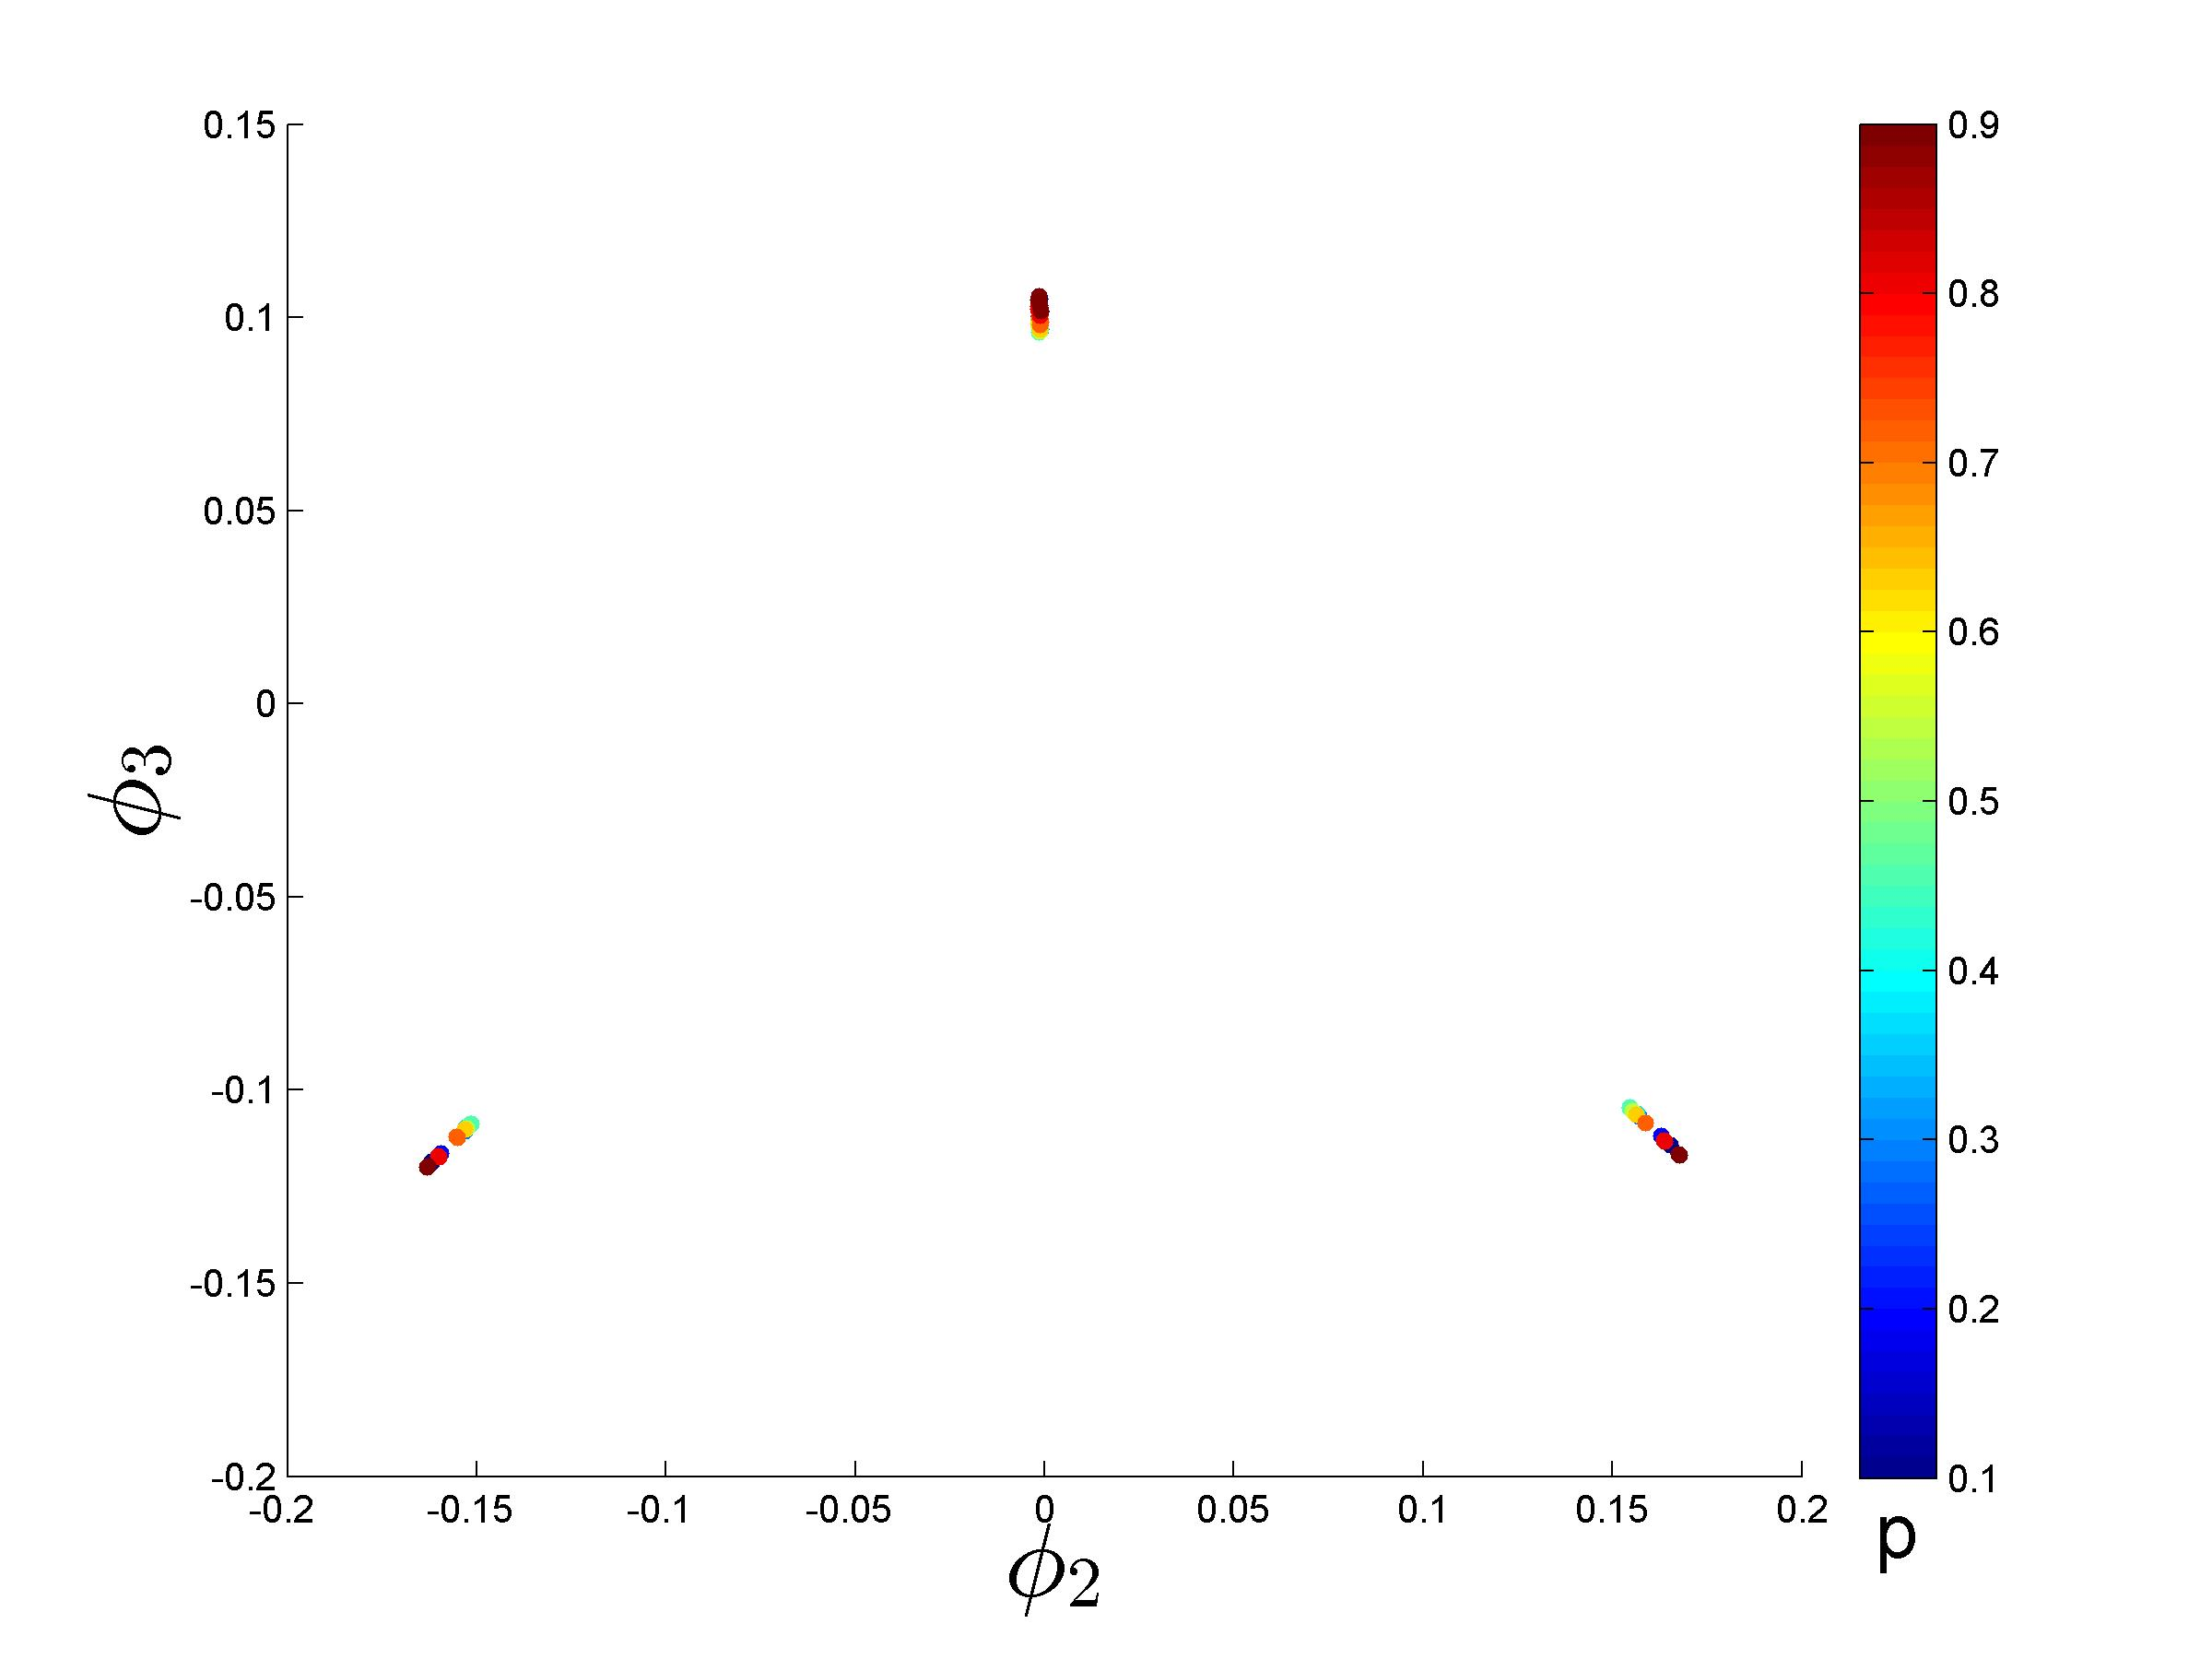
\includegraphics[width=\textwidth]{rawhist_p_1}
\caption{}
\end{subfigure}
\begin{subfigure}{0.2\textwidth}
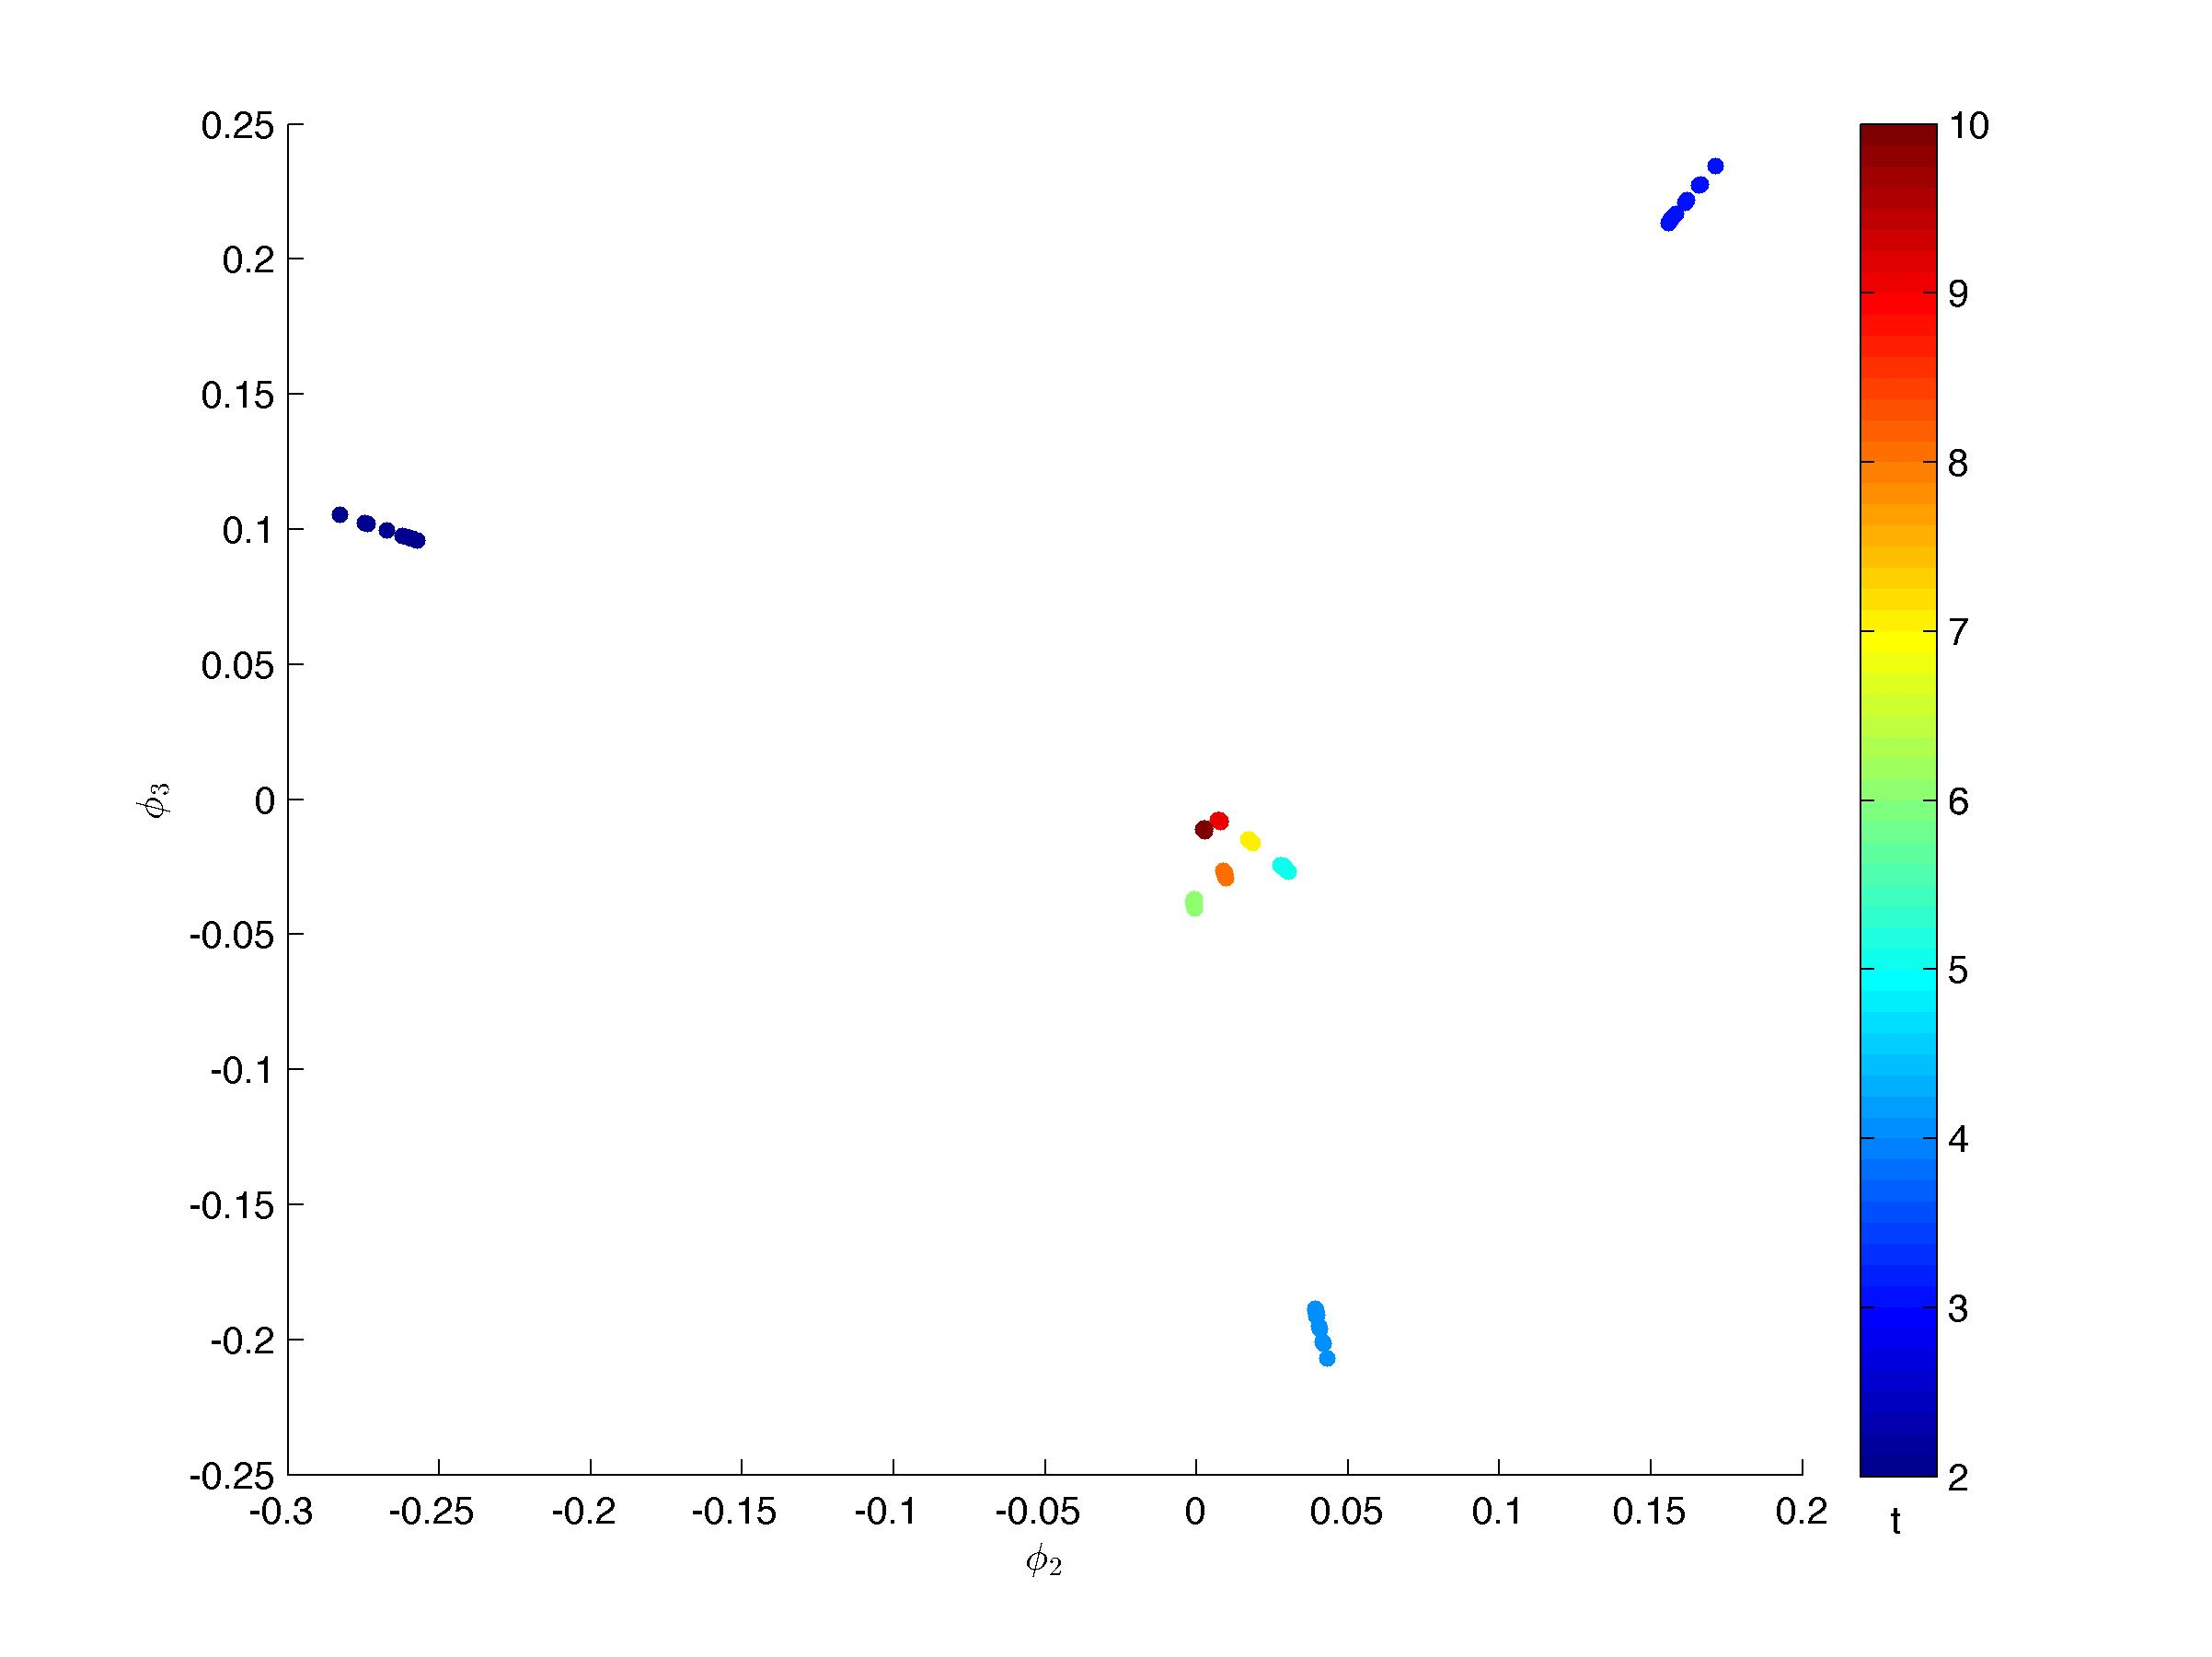
\includegraphics[width=\textwidth]{rawhist_t_1}
\caption{}
\end{subfigure}
\begin{subfigure}{0.2\textwidth}
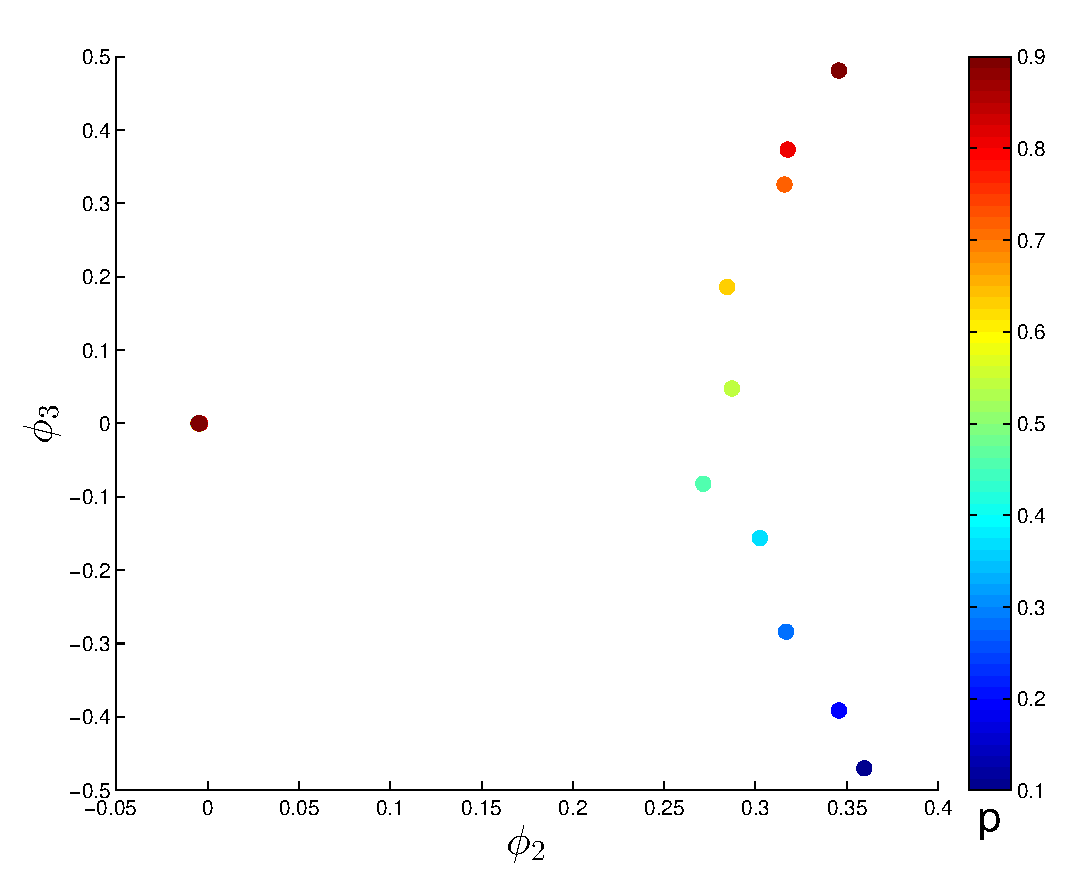
\includegraphics[width=\textwidth]{rawhist_p_400}
\caption{}
\end{subfigure}
\begin{subfigure}{0.2\textwidth}
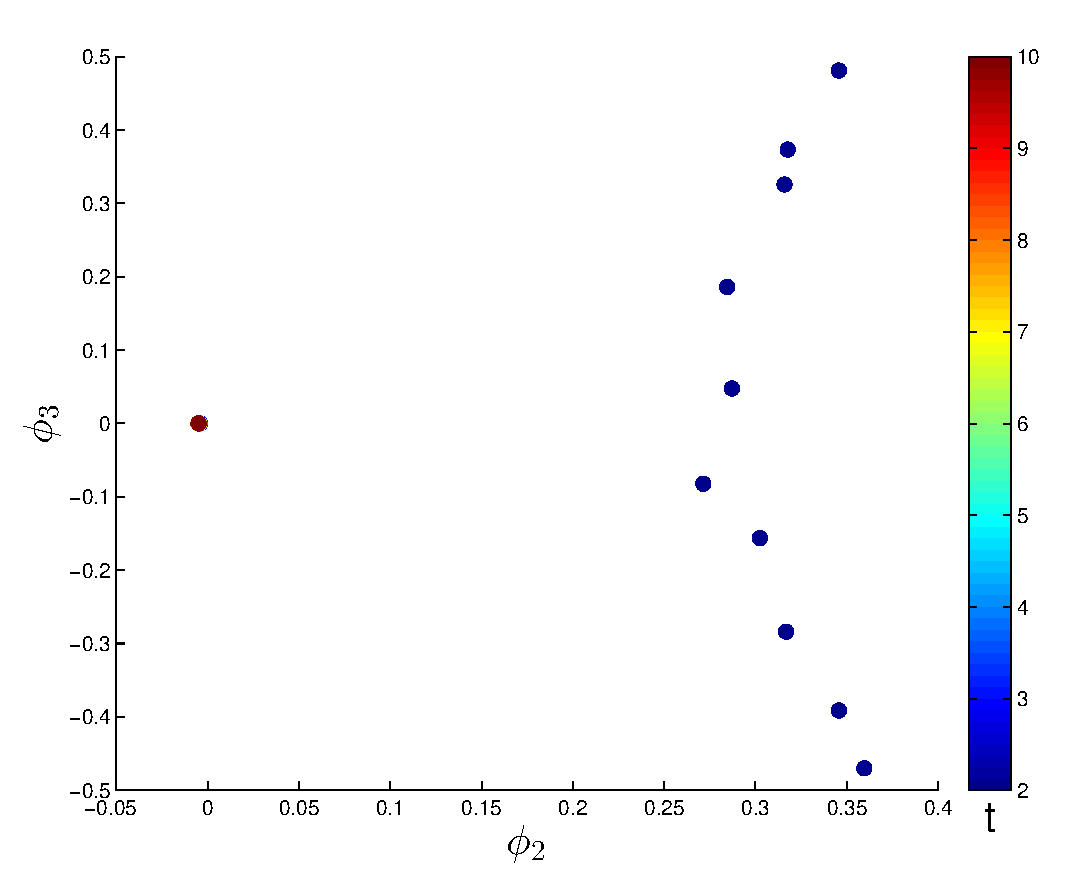
\includegraphics[width=\textwidth]{rawhist_t_400}
\caption{}
\end{subfigure}
\caption{Diffusion maps embeddings computed from simulation data of the velocity jump process with (a,b) $\lambda=1$, $s=1$, and (c,d) $\lambda=400$, $s=20$. The distances used in the diffusion maps kernel are the Euclidean distances between the histograms of particle positions. The data are colored by (a, c) $p$, the initial probability of a particle moving to the right, and (b, d) $t$, time.}
\label{fig:dmaps_embed_noemd}
\end{figure}
%TODO: for all figures - fix the labels of the axes - phi_2 vs. phi_1.

The second point we need to address is choosing appropriate distance metric between data points in \eqref{eq:W}.
%
Often, one uses the Euclidean distance between data points.
%
However, the Euclidean distance only considers the density at each bin and does not take into account the distance {\em between} bins.
%,such that two distributions whose supports are a short distance apart are closer (in norm) than two distributions whose supports are very far from each other.
%
%however, for histograms which approximate a probability density, the Euclidean distance can often be misleading.
%
%For example, the distance between two uniform distributions with finite, non-overlapping support will always be the same, {\em independent} of the distance between the support intervals.

To overcome this critical shortcoming, we propose to use the earth mover's distance (EMD) \cite{rubner2000earth} as our metric between histograms.
%
Conceptually, EMD measures how much ``work'' it takes to transform one probability density into another.
%
It therefore not only considers where the densities are inconsistent, but also how far apart the inconsistencies are.
%
Although the brute-force computation of the EMD is computationally expensive, there has been a plethora of work in developing efficient algorithms for the computation of EMD \cite{Pele-eccv2008, Pele-iccv2009}.
%
%TODO: we need to pay a special attention to the implementation of the EMD. We need to make it cleat that this distance can be very efficiently implemented  and therefore it is suitable for the practical uses and algorithm that we propose here as a viable tool for dynamical system analysis.
%
%For example, the EMD algorithm from \cite{Pele-eccv2008, Pele-iccv2009}....
%
%The implementation is available at \url{http://www.cs.huji.ac.il/~ofirpele/FastEMD/code}. 
For the special case of one-dimensional data, the EMD is equivalent to the $L_1$-norm between the cumulative distribution functions \cite{rubner2000perceptual}.
%\begin{equation}
%\| \rho_1  - \rho_2 \|_{EMD} = \int_{-\infty}^{\infty} \left| \int_{-\infty}^x \rho_1(y) dt - \int_{-\infty}^x \rho_2(y) dy \right| dx
%\end{equation}
%where $\rho_1(x)$ and $\rho_2(x)$ are two probability distributions defined on $x \in \mathbb{R}$. 
%
This can be estimated using histograms, 
\begin{equation}
\| z(i) - z(j) \|_{EMD} = \sum_{l=1}^{n} \left| \sum_{k=1}^l z_k(i) - \sum_{k=1}^l z_k(j) \right|
\end{equation}
where $z(i), z(j) \in \mathbb{R}^n$ are two histograms defined on (equally-spaced) bins in $\mathbb{R}$. 
%\section{Results}

%We simulate this stochastic velocity jump process for $N=1000$ particles, and $p \in [0.1, 0.9]$.
%%
%We simulate the process for $t \in [0, 10]$, and record the positions of each particle at uniform/equal time intervals.
%%
%We discard the initial portion of the trajectory corresponding to $t < 1$, as this is very noisy and corresponds to initial relaxation of the system.
%%
%We will consider two sets of simulations.
%%
%In one set, $\lambda = 1$ and $s=1$, and in the other set, $\lambda = 400$, and $s=20$.


%In Figure \ref{fig:dmaps_embed_noemd}, we have used the standard Euclidean distance between the histograms to compute the distances for \eqref{eq:W}.
%%
%The embeddings obtained are not particularly informative, and do not accurrately capture the underlying system dynamics.
%%
%This is due to our poor choice of metric, which does not accurrately describe the distances between histograms.

\begin{figure}[t]
\begin{subfigure}{0.45\columnwidth}
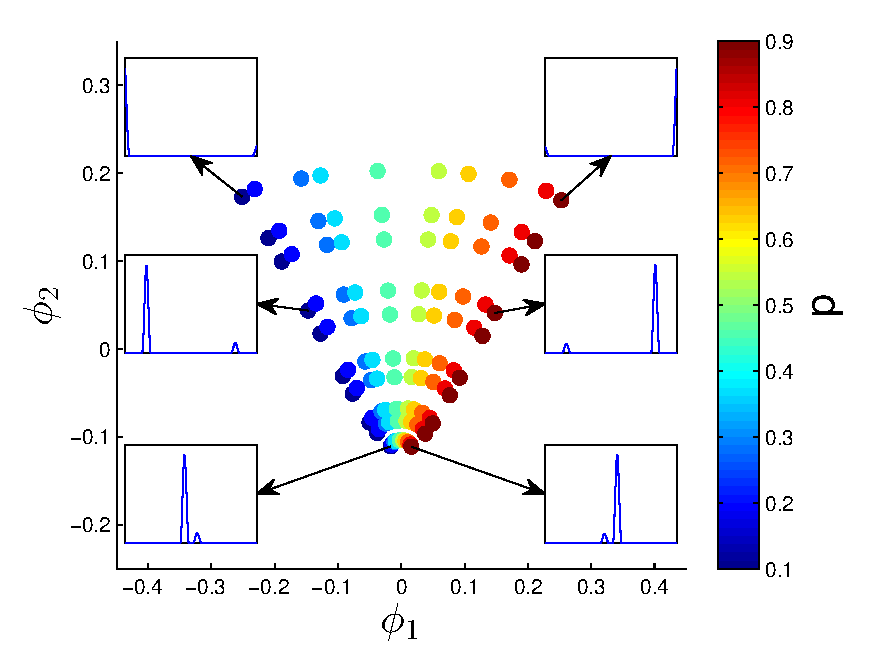
\includegraphics[width=\textwidth]{EMD_withhist_p_1}
\caption{}
\label{subfig:small_lambda_p}
\end{subfigure}
\begin{subfigure}{0.45\columnwidth}
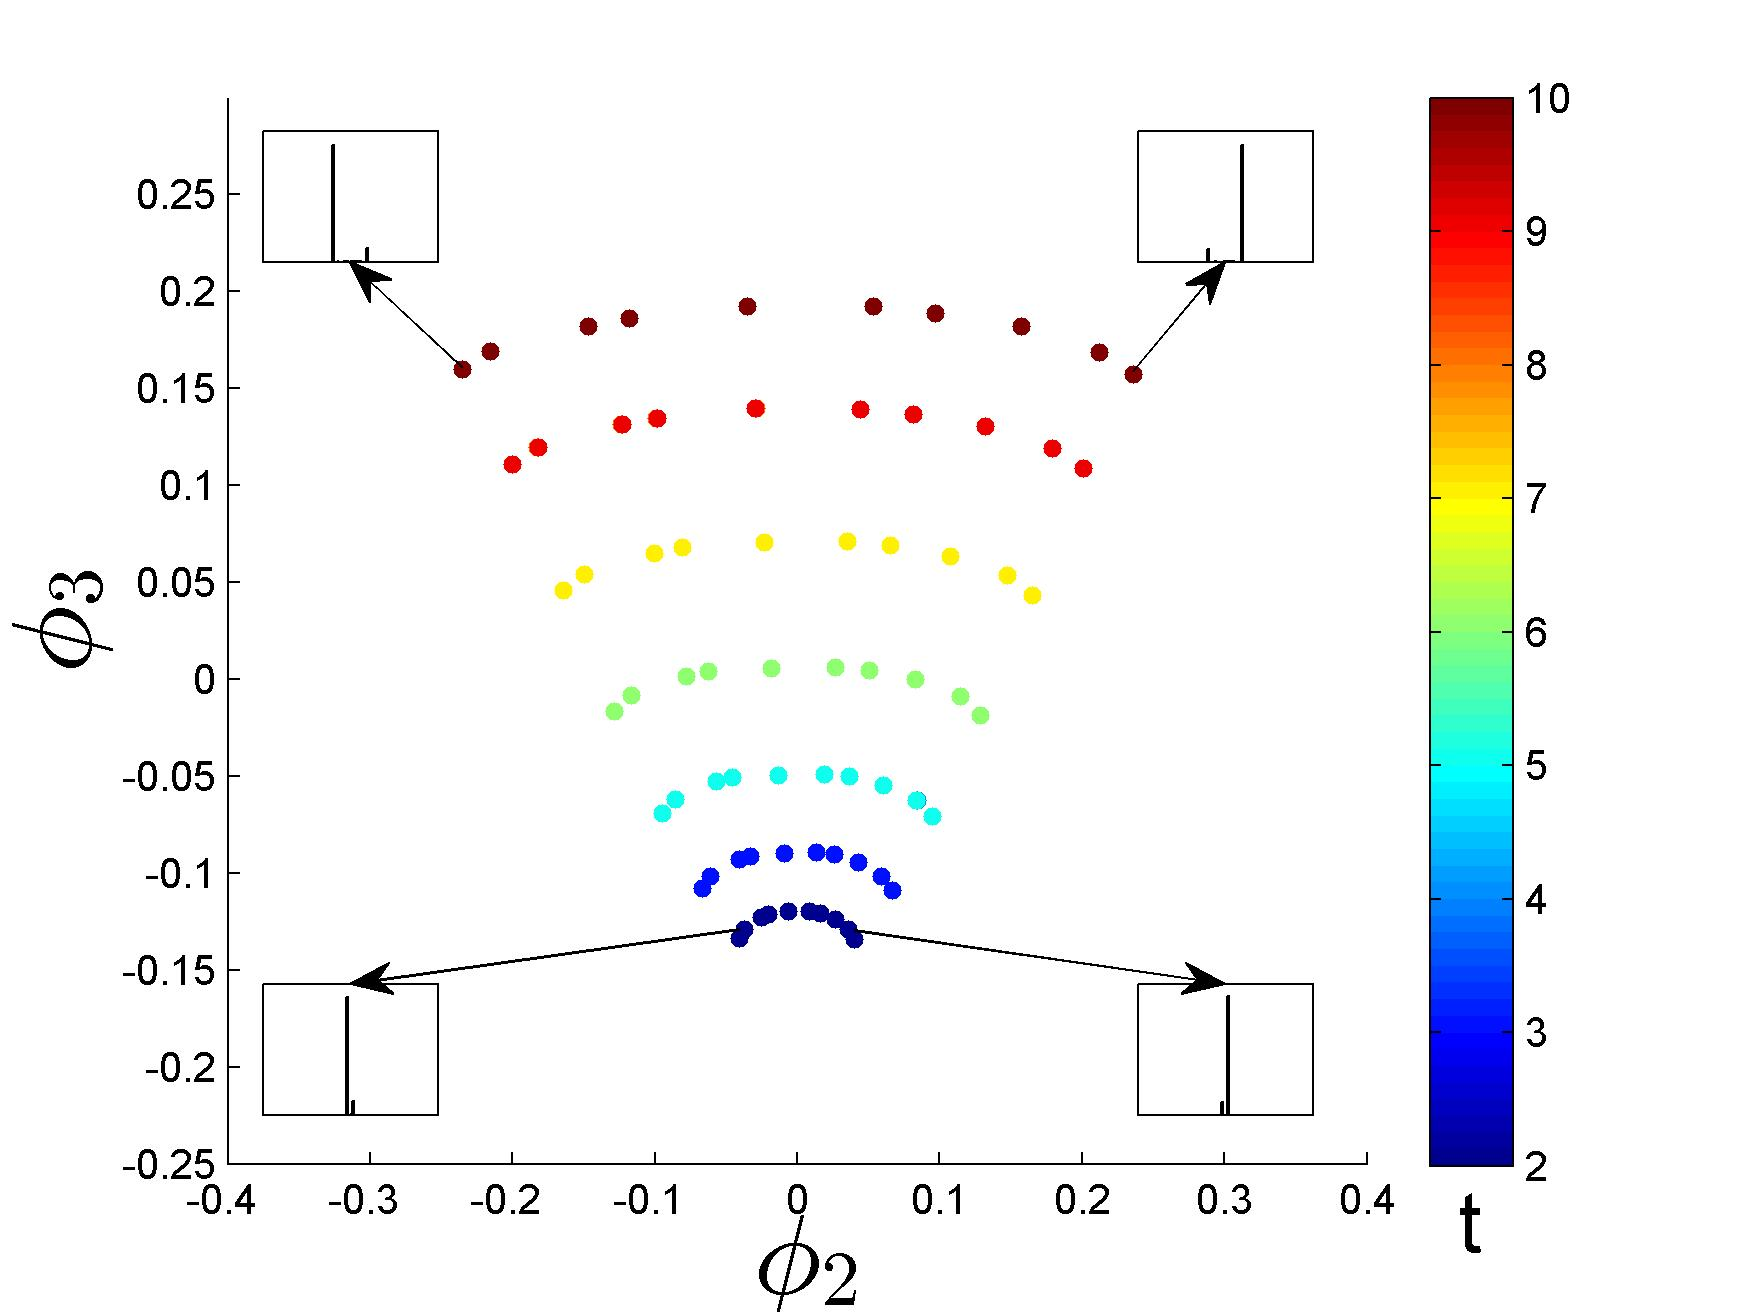
\includegraphics[width=\textwidth]{EMD_withhist_t_1}
\caption{}
\label{subfig:small_lambda_t}
\end{subfigure}
\begin{subfigure}{0.45\columnwidth}
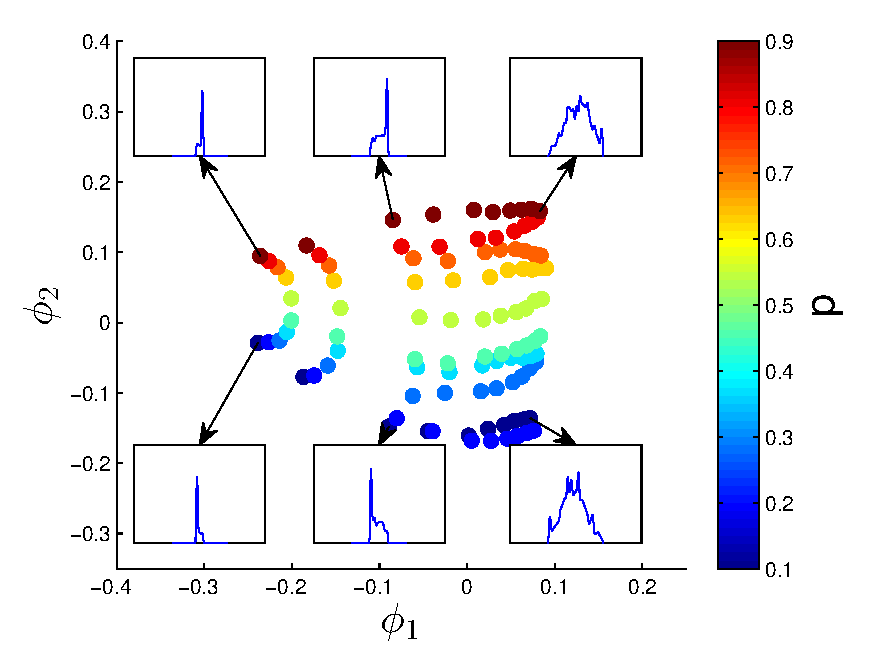
\includegraphics[width=\textwidth]{EMD_withhist_p_400}
\caption{}
\label{subfig:large_lambda_p}
\end{subfigure}
\begin{subfigure}{0.45\columnwidth}
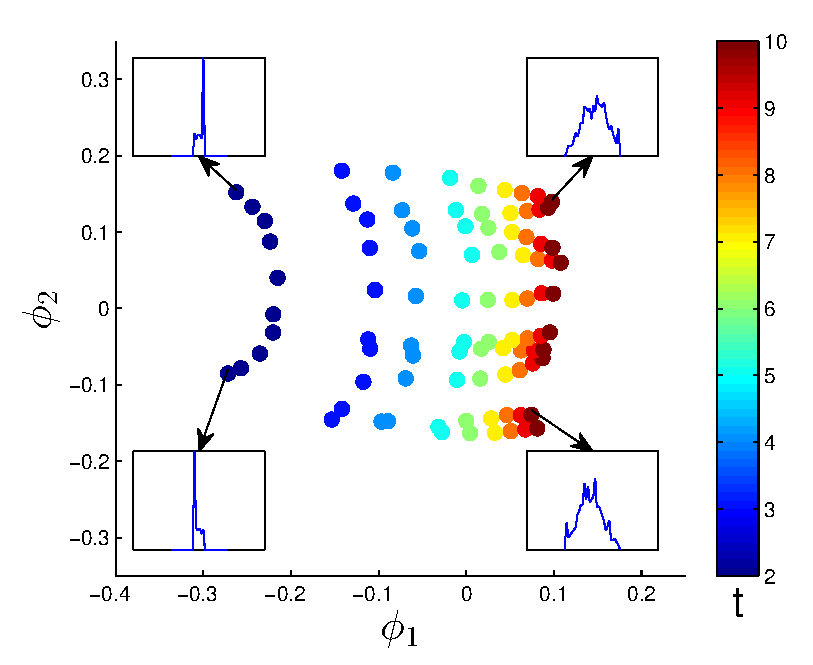
\includegraphics[width=\textwidth]{EMD_withhist_t_400}
\caption{}
\label{subfig:large_lambda_t}
\end{subfigure}
\caption{Diffusion maps embeddings computed from simulation data of the velocity jump process with (a,b) $\lambda=1$, $s=1$, and (c,d) $\lambda=400$, $s=20$. The distances used in the diffusion maps kernel are the earth mover's distances between the histograms of particle positions. The data are colored by (a, c) $p$, the initial probability of a particle moving to the right, and (b, d) $t$, time. Representative histograms are shown for selected data points.}
\label{fig:dmaps_embed_emd}
\end{figure}

We simulate the dynamics of this stochastic system to obtain our microscopic data to which we apply diffusion maps based on histograms and the EMD.
%
We consider two sets of simulations;
in one set (small $\lambda$), $\lambda = 1$ and $s=1$, and in the other set (large $\lambda$), $\lambda = 400$, and $s=20$.
%
For each set, we run many simulations, each with $N=1000$ particles.
%
We vary the initial condition of each simulation such that $0.1 \le p  \le 0.9$, and allow each simulation to evolve for $10$ time units.
%
We discard the initial portion of each simulation trajectory corresponding to $t < 1$, as this is very noisy and corresponds to initial relaxation of the system.

In Figure \ref{fig:dmaps_embed_noemd}, we have computed the diffusion maps embeddings of our two sets of simulation data, used the standard Euclidean distance between the histograms to compute the distances in \eqref{eq:W}.
%
The embeddings are not particularly informative and do not capture the underlying system dynamics; there is no strong correlation of the embedding coordinates with $p$ or $t$. 
%
This is due to our poor choice of metric, which does not accurately describe the distances between histograms.

In Figure \ref{fig:dmaps_embed_emd}, we have used the earth mover's distance to compute the distances between histograms.
%
The two system variables, $p$ and $t$, are well-correlated with the first two diffusion maps coordinates, $\phi_1$ and $\phi_2$. 
%
However, the ``more important'' coordinate, $\phi_1$, is correlated with $p$ for the small $\lambda$ case (Figure~\ref{subfig:small_lambda_p}), and correlated with $t$ for the large $\lambda$ case (Figure~\ref{subfig:large_lambda_t}); 
this is consistent with the macroscopic PDE description.
%
Furthermore, in the small $\lambda$ regime (wave equation), shown in Figures \ref{subfig:small_lambda_p} and \ref{subfig:small_lambda_t}, the points corresponding to small times are more clustered than the points corresponding to large times.
%
This is not surprising; at small times, the particles are more condensed around $x=0$, and it is more difficult to distinguish the particles moving to the left from the particles moving to the right. 
%
On the other hand, for large time, once the particles evolve from the origin, this separation is clear.  
%
For the large $\lambda$ case (heat equation), shown in Figures \ref{subfig:large_lambda_p} and \ref{subfig:large_lambda_t}, we observe that for small time the initial distribution $p$ is well organized in the embedding in Figure \ref{subfig:large_lambda_p}, since for small time the distribution of the particles is skewed and the initial velocity plays a role in this regime. 
%
On the other hand, for large time, we observe that the initial distribution $p$ is less organized in Figure \ref{subfig:large_lambda_p}, since the velocities have equilibrated and the initial distribution is less detectable in the particle density.

\begin{figure}[t]
\begin{subfigure}{0.45\columnwidth}
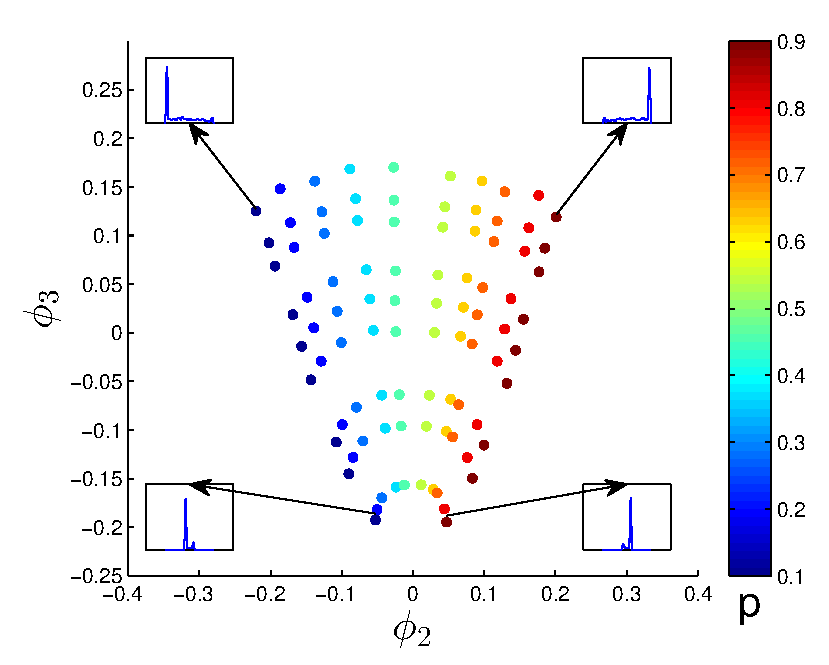
\includegraphics[width=\textwidth]{EMD2_withhist_p_10}
\caption{}
\end{subfigure}
\begin{subfigure}{0.45\columnwidth}
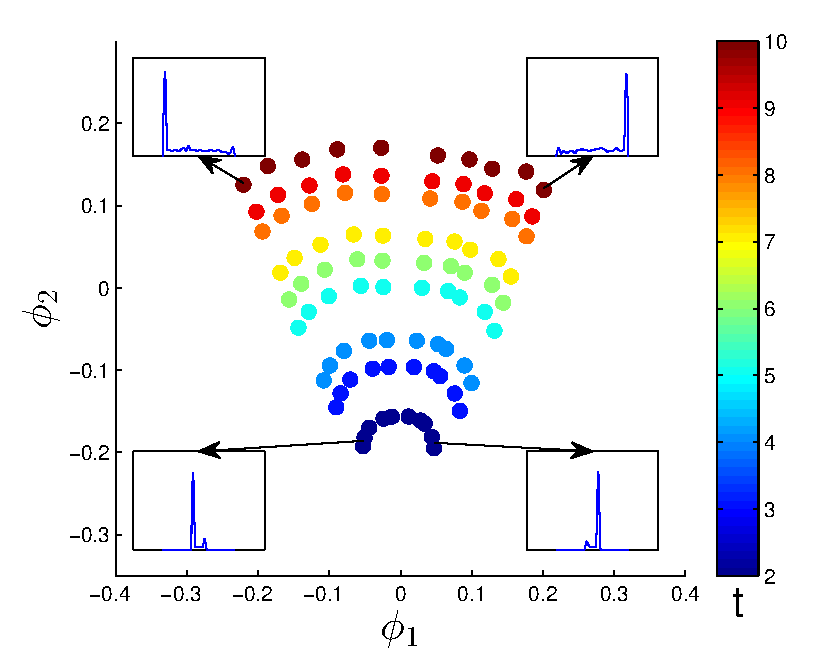
\includegraphics[width=\textwidth]{EMD2_withhist_t_10}
\caption{}
\end{subfigure}
\begin{subfigure}{0.45\columnwidth}
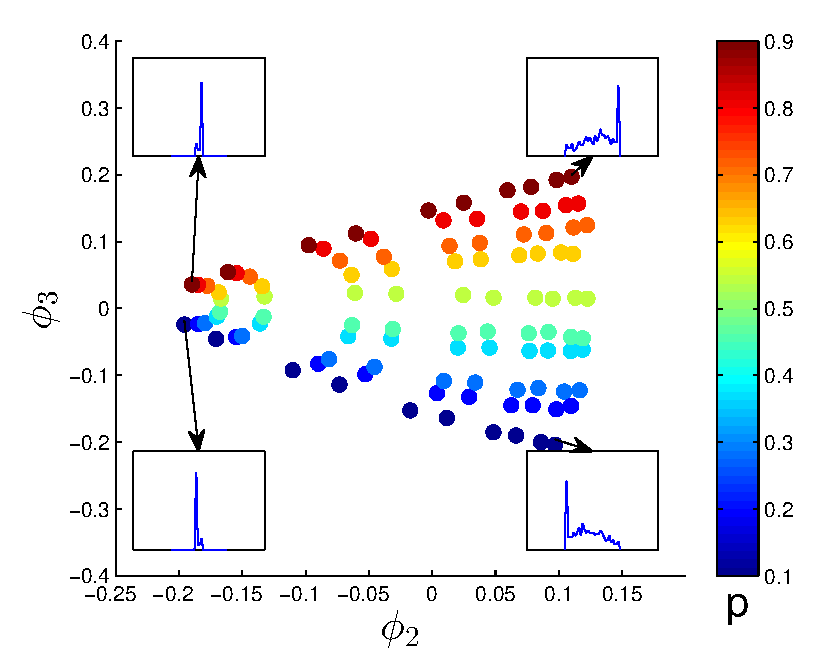
\includegraphics[width=\textwidth]{EMD2_withhist_p_20}
\caption{}
\end{subfigure}
\begin{subfigure}{0.45\columnwidth}
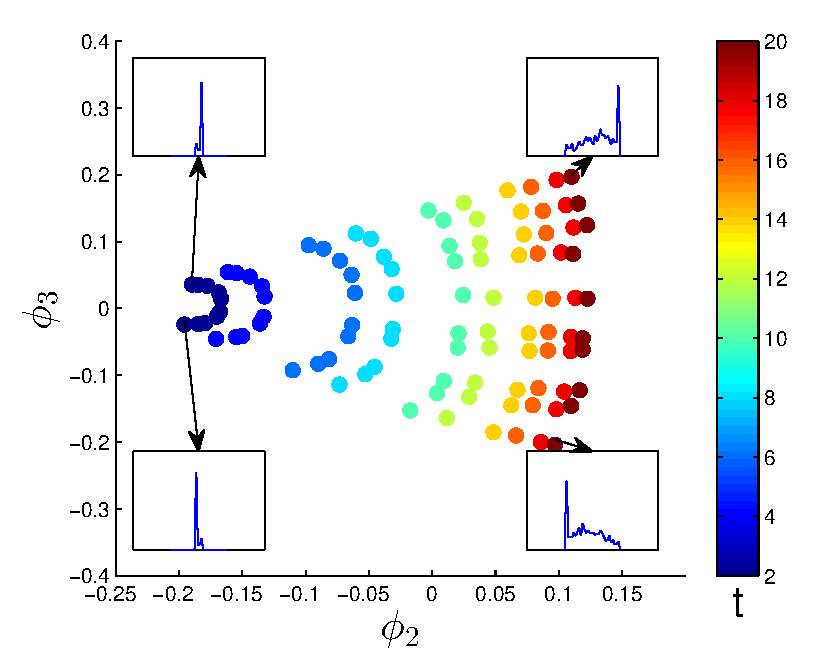
\includegraphics[width=\textwidth]{EMD2_withhist_t_20}
\caption{}
\end{subfigure}
\caption{Diffusion maps embeddings computed from simulation data of the velocity jump process with $\lambda=100$, $s=10$. The distances used in the diffusion maps kernel are the earth mover's distances between the histograms of particle positions. The data are colored by (a, c) $p$, the initial probability of a particle moving to the right, and (b, d) $t$, time. The particles are allowed to evolve for (a, b) 10 time units, and (c, d) 20 time units.  Representative histograms are shown for selected data points.} 
\label{fig:dmaps_embed_varyt}
\end{figure}

We have illustrated that diffusion maps can elucidate the relative importance of different system variables as a function of $\lambda$.
%
For the plots shown in Figure~\ref{fig:dmaps_embed_emd}, we can easily see the crossover from the wave-equation regime, where $p$ is more important, to the heat-equation regime, where $t$ is more important. 
%
However, we would like to note that this crossover point depends not only on $\lambda$, but also on the timescale of observation.
%
We can see this from our PDE description in \eqref{eq:second_order_pde};
clearly, $\lambda$ is defined relative to $t$, and so we should not only consider $\lambda$ in our analysis, but also the timescale of observation.
%
We can also detect this using diffusion maps to analyze our microscopic simulations.
%
We chose an intermediate value of $\lambda$ ($\lambda=100$ and $s=10$), and allowed the system to evolve for 10 and 20 time units. 
%
The results are shown in Figure \ref{fig:dmaps_embed_varyt}.
%
When the system only evolves for 10 time units, the majority of the data still appears ``wave-like'', and so the dominant parameter, $\phi_1$, is correlated with $p$, the initial condition.
%
However, when the system evolves for 20 time units, the initial velocity distribution has had more time to equilibrate - the behavior is more diffusive and $\phi_1$ is now correlated with $t$. 
%
Therefore, we can also see the crossover from wave-like behavior to heat-like behavior as a function of the observation timescale using diffusion maps.

We have presented algorithms to automatically uncover the variables which govern the macroscopic behavior of a system from data sampled at the microscopic level.
%
The essential components for our algorithms are choosing the correct observers and selecting the appropriate metric between these observers.
%
In our specific example, we used histograms of particle positions and the earth mover's distance between pairs of histograms.
%
With these two considerations, we used diffusion maps to uncover the two variables which characterize the system dynamics.
%
Furthermore, these two variables have a completely different nature;
one variable, $p$, characterizes the initial conditions of the system, whereas the other variable, $t$, describes the ``step-by-step'' evolution of the particles. 
%
This promotes the broad applicability of our methods to a wide variety of dynamical systems. 


%\section{Discussion}


%\bibliography{../../references/references}

\end{document}